\documentclass[12pt]{report}
\usepackage[spanish,es-nosectiondot,es-lcroman]{babel}
\usepackage{siunitx}
\usepackage[utf8]{inputenc}
\usepackage{amsmath}
\usepackage{float}
\usepackage{listings}
\usepackage{xcolor}
\usepackage{amssymb}
\usepackage{graphicx}
\usepackage{hyperref}
\usepackage{geometry}
\usepackage[backend=biber,style=ieee]{biblatex}
\addbibresource{./citas/citas.bib}
%Configuracion para el . en decimales
\sisetup{output-decimal-marker = {.}}
% Configuración para el código
\lstset{
	language=Python,
	basicstyle=\ttfamily\footnotesize,
	numbers=left,
	numberstyle=\tiny\color{gray},
	stepnumber=1,
	numbersep=10pt,
	backgroundcolor=\color{white},
	showspaces=false,
	showstringspaces=false,
	showtabs=false,
	frame=single,
	rulecolor=\color{black},
	tabsize=4,
	captionpos=b,
	breaklines=true,
	breakatwhitespace=false,
	linewidth=\linewidth,
	keepspaces=true,
	columns=flexible,
	keywordstyle=\bfseries\color{blue},
	commentstyle=\itshape\color{lightgray},
	stringstyle=\color{red},
	escapeinside={\%*}{*)},
}

% Configuración de los márgenes
\geometry{
	left=2cm,   % Margen izquierdo
	right=2cm,  % Margen derecho
	top=2cm,    % Margen superior
	bottom=2cm  % Margen inferior
}

% Title Page
\title{
	\begin{center}
		Machine Learning para mineria de datos\\
		Homework 2
		
	\end{center}
}
\author{Salazar Martinez Miguel Angel}
\begin{document}
	\renewcommand{\arraystretch}{1.3}
	
	\maketitle
	
\begin{figure}[H]
	\centering
	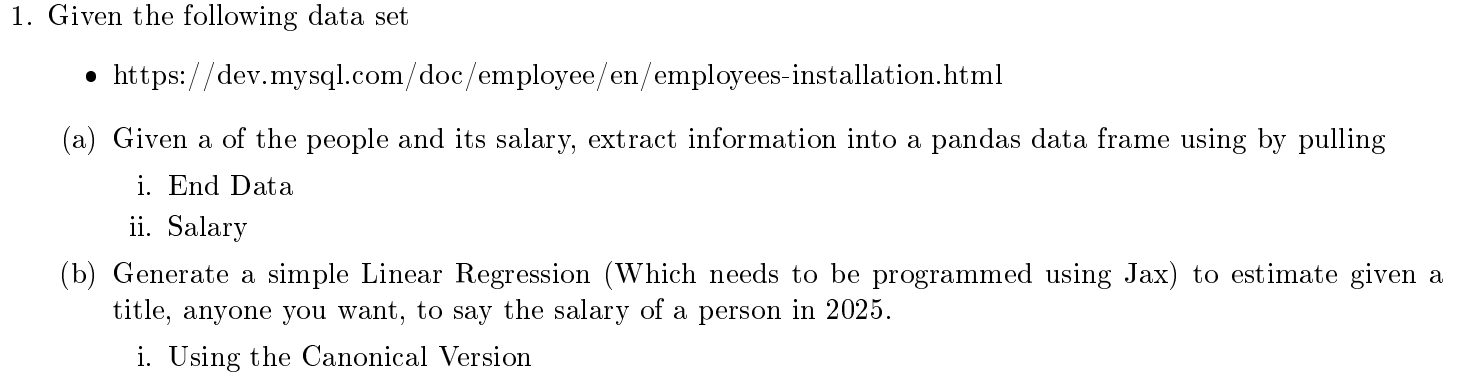
\includegraphics[width=1\textwidth]{screenshot001}
\end{figure}

\begin{figure}[H]
	\centering
	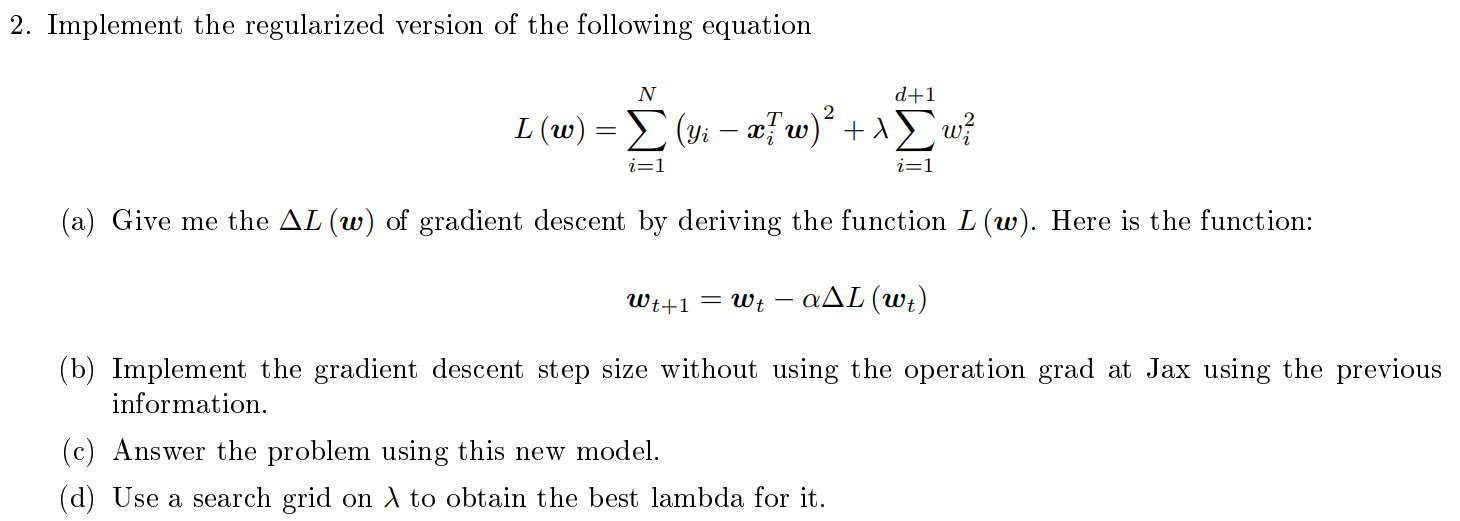
\includegraphics[width=1\textwidth]{screenshot002}
\end{figure}

\begin{figure}[H]
	\centering
	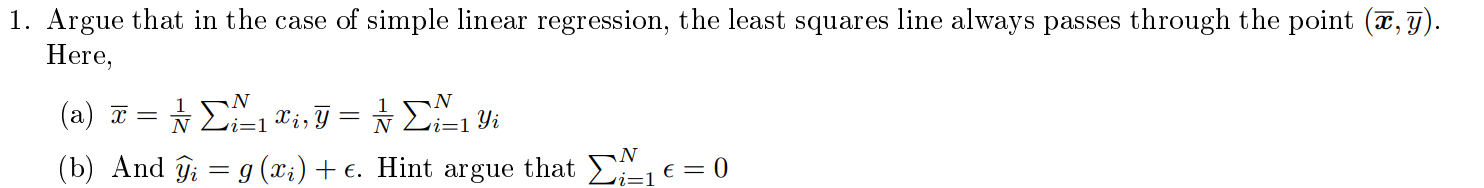
\includegraphics[width=1\textwidth]{screenshot003}
\end{figure}

\begin{figure}[H]
	\centering
	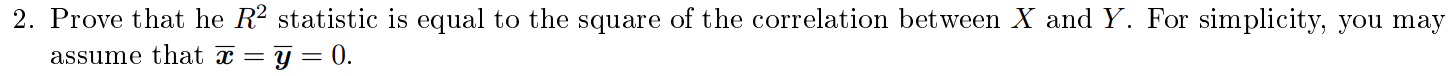
\includegraphics[width=1\textwidth]{screenshot004}
\end{figure}


\begin{figure}[H]
	\centering
	
\includegraphics[width=1\textwidth]{screenshot008}
\end{figure}

\begin{figure}[H]
	\centering
	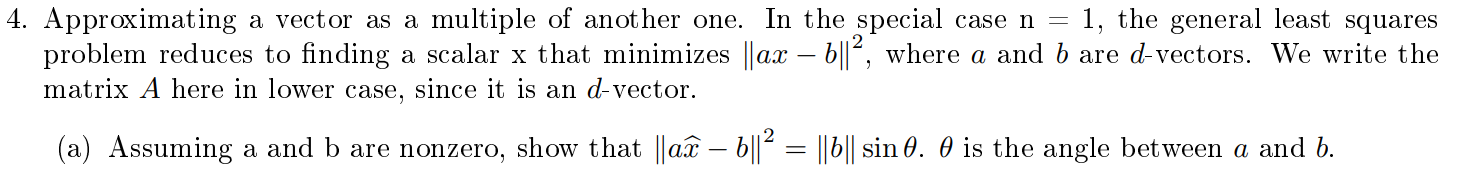
\includegraphics[width=1\textwidth]{screenshot006}
\end{figure}

\begin{figure}[H]
	\centering
	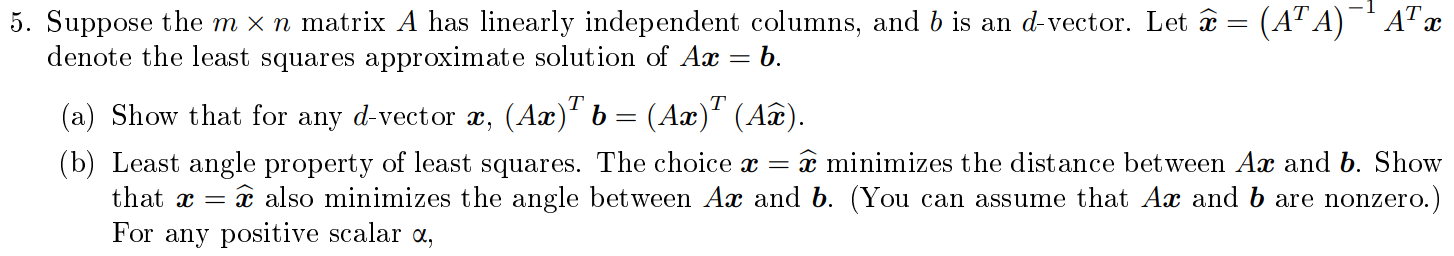
\includegraphics[width=1\textwidth]{screenshot007}
\end{figure}

\printbibliography
\end{document}	

